\chapter{Databasen}
Nedenfor følger design af software til databasen og dens interface. Dette er lavet på baggrund af kravspecifikation og systemarkitektur. 



\subsection{Modultes Ansvar}
Databasen er her hvor havne terminalens personale kan aflæse data fra skibet. Disse data er sendt fra KI. Programmerne indeholder brugergrænseflader der opfylder kravene, beskrevet i kravspecifikationen. Her kan der også ses en prototyper på brugergrænsefladen.
Database modulet har 3 dele. Severen, Web-siden og en mySQL database. \\
\textbf{Severen} står for kommunikationen immellem KI og Databasen. Severen modtager data fra KI og lager disse i en tekst fil\\
\textbf{Web-siden} giver brugeren mulighed for at se info om BROS samt at logge sig ind i BROS database hvorfra at data om skibe der er tilsluttet systemet kan aflæses. Web-sidens 3 vigtigste funktioner er at gemme ny data til mySQL databasen, slette den tekst fil som severen lavede og vise data for brugeren. Til at håndtere web-siden benyttes en apache server.
\textbf{mySQL databasen} er en database som er  installeret på computeren. Alle data som er sendt fra KI er lageret i mySQL databasen.

\subsection{Klassediagrammer}
Nedenfor ses klassediagrammerne for databasen. Bemærk database modulet er lavet som en server del og en web del
\begin{figure}[H]
	\centering
	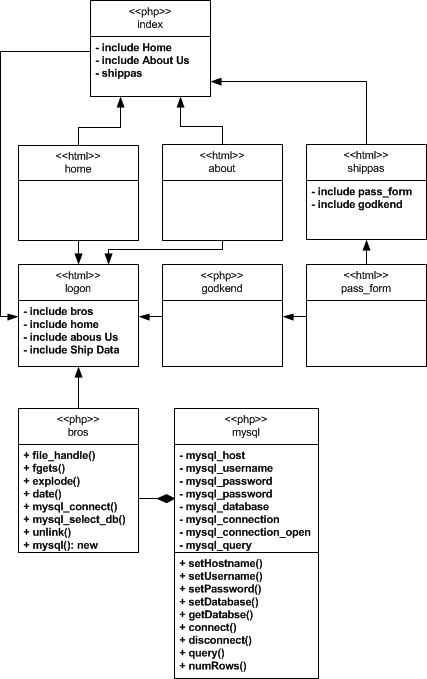
\includegraphics[width=0.8\textwidth]{billeder/web_klasse}
	\caption{Klassedigram for databasens severer}
	\label{fig:serverKlassediagram}
\end{figure}
\fixme{skal laves om, snakket med KIM}

tilføj dato()
\begin{figure}[htbp]
	\centering
	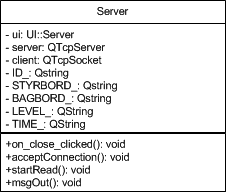
\includegraphics[width=0.3\textwidth]{billeder/serverKlassediagram}
	\caption{Klassedigram for databasens severer}
	\label{fig:serverKlassediagram}
\end{figure}

\subsection{Globale variabler}


\subsection{Funktionsbeskrivelser}
\subsubsection{Server}
Denne header har til ansvar at starte GUI og håndtere TCP forbindelse\\

\begin{table}[H]
\begin{tabular}{l p{12.5cm}}
\multicolumn{2}{l}{\texttt{\textcolor{blue}{Void} on\_close\_clicked( \textcolor{blue}{void} )}} \\
\hline
Beskrivelse:&Ved klik forespørges brugeren om denne ønsker at lukke severen\\
Parametre:&\\
Returværdi:&\\
\end{tabular}
\end{table}

\begin{table}[H]
\begin{tabular}{l p{12.5cm}}
\multicolumn{2}{l}{\texttt{\textcolor{blue}{Void} acceptConnection( \textcolor{blue}{void} )}} \\
\hline
Beskrivelse:&Står for at acceptere forbindelse fra KI og connecte.\\
Parametre:&QTcpServer server\\
				&QTcpSocket* client\\
Returværdi:&\\
\end{tabular}
\end{table}

\begin{table}[H]
\begin{tabular}{l p{12.5cm}}
\multicolumn{2}{l}{\texttt{\textcolor{blue}{Void} startRead( \textcolor{blue}{void} )}} \\
\hline
Beskrivelse:&Læser data fra socket. Data til fil og GUI\\
Parametre:&QTcpSocket* client\\
Returværdi:&\\
\end{tabular}
\end{table}

\subsubsection{Wep-side}
Web-siden står for at fremvise skibs data grafisk for terminal personalet. Desuden står den for at lager data og loade data fra mySQL databasen.\\

\subsubsection{bros}

\begin{table}[H]
\begin{tabular}{l p{12.5cm}}
\multicolumn{2}{l}{\texttt{\textcolor{blue}{} file\_handle( \textcolor{blue}{} )}} \\
\hline
Beskrivelse:&Læse hvilken adresse databasen ligger på\\
Parametre:&\\
Returværdi:&\\
\end{tabular}
\end{table}

\begin{table}[H]
\begin{tabular}{l p{12.5cm}}
\multicolumn{2}{l}{\texttt{\textcolor{blue}{} fgets ( \textcolor{blue}{} )}} \\
\hline
Beskrivelse:&Læse hvilken adresse databasen ligger på\\
Parametre:&\\
Returværdi:&\\
\end{tabular}
\end{table}

\begin{table}[H]
\begin{tabular}{l p{12.5cm}}
\multicolumn{2}{l}{\texttt{\textcolor{blue}{} explode( \textcolor{blue}{} )}} \\
\hline
Beskrivelse:&Læse hvilken adresse databasen ligger på\\
Parametre:&\\
Returværdi:&\\
\end{tabular}
\end{table}

\begin{table}[H]
\begin{tabular}{l p{12.5cm}}
\multicolumn{2}{l}{\texttt{\textcolor{blue}{} mysql\_connect( \textcolor{blue}{} )}} \\
\hline
Beskrivelse:&Læse hvilken adresse databasen ligger på\\
Parametre:&\\
Returværdi:&\\
\end{tabular}
\end{table}

\begin{table}[H]
\begin{tabular}{l p{12.5cm}}
\multicolumn{2}{l}{\texttt{\textcolor{blue}{} mysql\_select\_db( \textcolor{blue}{} )}} \\
\hline
Beskrivelse:&Læse hvilken adresse databasen ligger på\\
Parametre:&\\
Returværdi:&\\
\end{tabular}
\end{table}

\begin{table}[H]
\begin{tabular}{l p{12.5cm}}
\multicolumn{2}{l}{\texttt{\textcolor{blue}{} unlink( \textcolor{blue}{} )}} \\
\hline
Beskrivelse:&Læse hvilken adresse databasen ligger på\\
Parametre:&\\
Returværdi:&\\
\end{tabular}
\end{table}

\begin{table}[H]
\begin{tabular}{l p{12.5cm}}
\multicolumn{2}{l}{\texttt{\textcolor{blue}{new} mysql( \textcolor{blue}{} )}} \\
\hline
Beskrivelse:&Læse hvilken adresse databasen ligger på\\
Parametre:&\\
Returværdi:&\\
\end{tabular}
\end{table}

\subsubsection{mysql}
\begin{table}[H]
\begin{tabular}{l p{12.5cm}}
\multicolumn{2}{l}{\texttt{\textcolor{blue}{} setHostName( \textcolor{blue}{} )}} \\
\hline
Beskrivelse:&Læse hvilken adresse databasen ligger på\\
Parametre:&\\
Returværdi:&\\
\end{tabular}
\end{table}

\begin{table}[H]
\begin{tabular}{l p{12.5cm}}
\multicolumn{2}{l}{\texttt{\textcolor{blue}{} setUserName( \textcolor{blue}{} )}} \\
\hline
Beskrivelse:&Skriver brugernavn til databasen\\
Parametre:&\\
Returværdi:&\\
\end{tabular}
\end{table}

\begin{table}[H]
\begin{tabular}{l p{12.5cm}}
\multicolumn{2}{l}{\texttt{\textcolor{blue}{} setPassword( \textcolor{blue}{} )}} \\
\hline
Beskrivelse:&Skriver password til databasen\\
Parametre:&\\
Returværdi:&\\
\end{tabular}
\end{table}

\begin{table}[H]
\begin{tabular}{l p{12.5cm}}
\multicolumn{2}{l}{\texttt{\textcolor{blue}{} setDatabase( \textcolor{blue}{} )}} \\
\hline
Beskrivelse:&Fortæller mySQL hvilken database der skal benyttes\\
Parametre:&\\
Returværdi:&\\
\end{tabular}
\end{table}

\begin{table}[H]
\begin{tabular}{l p{12.5cm}}
\multicolumn{2}{l}{\texttt{\textcolor{blue}{} getDatabase( \textcolor{blue}{} )}} \\
\hline
Beskrivelse:Tager fat i databasen\\
Parametre:&\\
Returværdi:&\\
\end{tabular}
\end{table}

\begin{table}[H]
\begin{tabular}{l p{12.5cm}}
\multicolumn{2}{l}{\texttt{\textcolor{blue}{} connect( \textcolor{blue}{} )}} \\
\hline
Beskrivelse:&Står for at samle localhost, username, password, database og connecte til databasen\\
Parametre:&\\
Returværdi:&\\
\end{tabular}
\end{table}

\begin{table}[H]
\begin{tabular}{l p{12.5cm}}
\multicolumn{2}{l}{\texttt{\textcolor{blue}{} disconnect( \textcolor{blue}{} )}} \\
\hline
Beskrivelse:&Lukker database forbindelsen\\
Parametre:&\\
Returværdi:&\\
\end{tabular}
\end{table}

\begin{table}[H]
\begin{tabular}{l p{12.5cm}}
\multicolumn{2}{l}{\texttt{\textcolor{blue}{} query( \textcolor{blue}{} )}} \\
\hline
Beskrivelse:&Opretter database kø og skriver data til skærm\\
Parametre:&\\
Returværdi:&\\
\end{tabular}
\end{table}

\begin{table}[H]
\begin{tabular}{l p{12.5cm}}
\multicolumn{2}{l}{\texttt{\textcolor{blue}{} numRows( \textcolor{blue}{} )}} \\
\hline
Beskrivelse:&Checker hvor mange rækker der findes i databasen bruges desuden til at udskrive om databasen er tom.\\
Parametre:&\\
Returværdi:&\\
\end{tabular}
\end{table}

\section{Design}
\subsection{Server}
\begin{figure}[htbp]
	\centering
	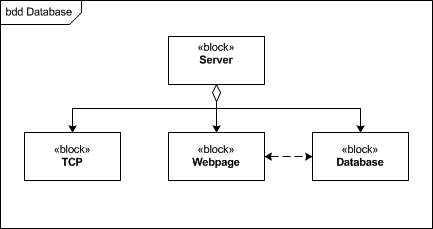
\includegraphics[width=0.6\textwidth]{billeder/bdd_server}
	\caption{BDD server}
	\label{fig:bdd_server}
\end{figure}

Databasen er en server som har de 3 underblokke TCP, Database og Web-page som illustreret på figur \ref{fig:bdd_server}

TCP er en dataforbindelse (Transmission Control Protocol). Denne protokol er benyttes til at sende data fra KI til serveren. Severen vil modtage data og lagere dette i en midlertidig backup fil. TCP-forbindelsen er kodet i C++.
For TCP-forbindelsen benyttes TCP - protocollen som tilbyder sikker data overførelse fra BROS.
Databasen er en mySQL database som frit kan downloades og installeres på en Linux, Windows eller Mac.
Man skal installere en server del og en client del. Server delen er den del der gør det muligt at håndtere og lagre data. Denne ligger under client delen og er nødvendig for at client kan fungere. mySQL client gør det muligt at en bruger kan tilgår og læse fra databsen uden at gør ændringer i denne. Dette benytte i web interfacet. mySQL kan tilgås direkte fra terminalen og giver mulighed for forskellige opsætninger af databaser og tabeller samt forskellige bruger rettigheder.
\textbf{mulighede med mySQL}
Web-pagen er udviklet i php som giver gode muligheder for kommunikation til og fra mySQL databasen. Web-pagen er implementeret ved hjælp af en apache server som er en web server. Web-pagen har en general information omkring BROS og et login til at tilgå databasen. Ved at anvende et web-interface gives der mulighe for at data kan aflæses fra andre pladser end fra den direkte server. Ved at kende ip eller host navn er det muligt at tilgå web-siden.
Den web baserede database loader mySQL databasen og fremviser denne grafisk for brugeren.

\subsection{TCP server}
\begin{figure}[htbp]
	\centering
	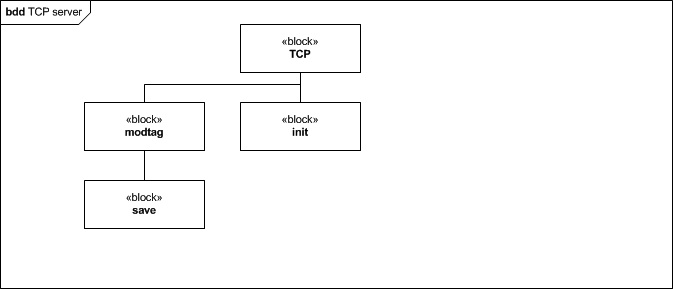
\includegraphics[width=0.5\textwidth]{billeder/bdd_TCP_server}
	\caption{BDD TCP server(ikke færdig)}
	\label{fig:bdd_TCP_server}
\end{figure}



TCP protocollen er en af kerneprotokollerne på nutidens internet. Gennem TCP kan forskellige værtsmaskine igennem f.eks. internet ethernet og trådet forbindelse oprette forbindelse til hinanden og udveksle datepakker. Protokollen giver programmelt på værtsmaksine nogle vitale garantier for at disse datapakker afsendes og modtages ved:
\begin{itemize}
	\item Stabilitet: En pakke der går tabt bliver forsøgt afsendt igen
	\item Ordnet levering: En pakke kommer frem til modtageren i samme rækkefølge som de blev afsendt
\end{itemize}
Der ud over benytter TCP sig af forskellige port numre. Forskellige portnumrer gør dte muligt etablere flere forskellige datstrømme til og fra samme værtsmaskine.

Selve programmet er kodet op over socket programmering. Under opstart initialiseres socket, ip og porte. Når disse er succesfuldt initialiseret afvendter TCP serveren at KI connecter. Efter connection modtager TCP serveren datapakken fra KI og gemmer denne i en textfil kaldt ship.txt. Denne fil bruges bruges som en midlertidig sikkerhed for at data fra KI sikkert bliver inført i mySQL databasen.

sequuens diagram

\subsection{Web-side}
\begin{figure}[htbp]
	\centering
	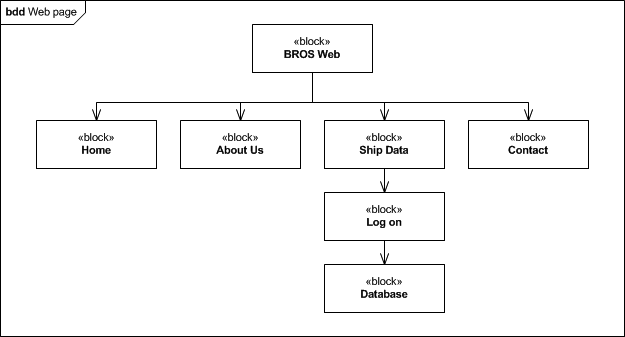
\includegraphics[width=0.8\textwidth]{billeder/bdd_web}
	\caption{BDD Web-page BROS}
	\label{fig:bdd_web}
\end{figure}

For at web siden kan køre kræves der at der på serveren er installeret en web - server. Der er på denne server installeret apache som web - server.\\
Ved opstart af serveren bliver denne automatisk startet og start siden er \textbf{BROS}. Web siden fungere som bruger interfacet for havne terminalen. Web siden er opbygget som et dynamisk web page og kodet i php. Dette sikre minmal loading time ved hjælp af ajax. Alle styles på siden er styret af css. Siden har 4 forskellige under sider Home, About Us, Ship Data og Contact. Ved klik på Ship Data vil man blive bedt om at taste sit password som sikre at kun autoriserede personer får adgang til systemet.\\
Siden der håndtere skibs data starter med at connecte til mySQL databasen om ikke der kan connectes til databasen vil der blive udskrevet en error og siden vil igen forsøge at conencte til databasen. Efter connection til databasen vil den gemte fil fra TCP-serveren blive loadet ind i mySQL databasen og filen vil blive slettet. efter loading vil siden loade alle data i mySQL databasen og vise denne for brugeren. Data der kan vises for brugeren er:
\begin{itemize}
	\item Skibs ID
	\item Højre tanks vandniveau
	\item Venstre tanks vandniveau
	\item Hældningsniveau
	\item Forbindelse til KI
\end{itemize}
Siden checker hvert 5 sekund om der er nu data. Hved ny data vil denne blvie placeret øverst på siden.
Når brugeren er færdig med at benytte BROS databasen kan brugeren trykke log of i øverste højre hjørne.

\section{Metodebeskrivelse}
\subsection{TCP KI}
\textbf{Void msg(string, string, string, string, string);}\\
Håndtere data der skal sendes via tcp.\\
\textbf{Void socket();}\\
Opretter socket forbindelse for ctp client.\\
\textbf{Void connection();}\\
Kalder ip adresse og portnummer for TCP server. Overføre data.\\

\subsection{TCP database}
\textbf{Void socketConnect();}\\
\textbf{Void msgServer();}\\




